\documentclass[../Main.tex]{subfiles}
\begin{document}

\section{Classical Reinforcement Learning Algorithms}

In this section, we explore the major classical methods used to solve reinforcement learning problems. These approaches vary based on whether they require a model of the environment, how they estimate value functions, and how they update policies. Understanding these foundational algorithms is crucial as they form the building blocks for modern deep reinforcement learning methods.

\subsection{Taxonomy of Reinforcement Learning Algorithms}

Reinforcement Learning algorithms can be categorized along several conceptual dimensions. Understanding this taxonomy helps clarify the assumptions, strengths, and use-cases of different methods.

\begin{figure}[h]
    \centering
    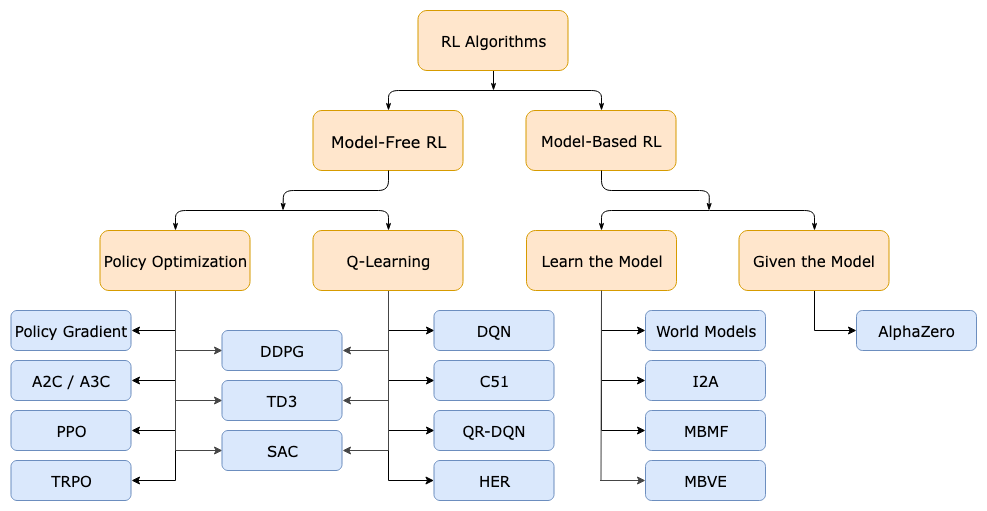
\includegraphics[width=1\textwidth]{img/RL-taxonomy.png}
    \caption{Illustrative taxonomy of RL algorithms across three axes.}
\end{figure}

\subsubsection{Model-based vs. Model-free:}
\begin{itemize}
    \item \textbf{Model-based RL:} The agent has access to, or learns, a model of the environment's dynamics (transition probabilities and rewards). Planning is performed via algorithms like Dynamic Programming or Model Predictive Control.
    \item \textbf{Model-free RL:} The agent learns directly from interactions with the environment, without an explicit model. This includes methods like Monte Carlo, Temporal Difference Learning, and Deep Q-Learning.
\end{itemize}

\subsubsection{Value-based vs. Policy-based vs. Actor-Critic:}
\begin{itemize}
    \item \textbf{Value-based:} Learn a value function (e.g., Q-values), and derive the policy implicitly. Examples: Q-learning, DQN.
    \item \textbf{Policy-based:} Learn the policy directly, typically via gradient ascent on expected return. Examples: REINFORCE, PPO.
    \item \textbf{Actor-Critic:} Combine both approaches; an actor updates the policy, and a critic estimates the value function.
\end{itemize}

\subsubsection{Planning vs. Learning:}
\begin{itemize}
    \item \textbf{Planning:} Uses a known or learned model to simulate outcomes and plan actions. Example: Value Iteration.
    \item \textbf{Learning:} Updates knowledge (value functions or policies) directly from experience. Example: Sarsa, DQN.
\end{itemize}

This taxonomy helps structure our study of RL. In the following sections, we start with model-based methods such as Dynamic Programming, then proceed to model-free approaches like Monte Carlo, TD learning, and their deep variants.

\subsection{Dynamic Programming (DP)}

Dynamic Programming uses the Bellman equations to compute value functions and derive optimal policies, assuming a complete model of the environment's dynamics is available \cite{bellman1957dynamic}.

\subsubsection{Key Assumptions and Properties:}
\begin{itemize}
    \item Requires access to the transition probabilities $P(s'|s, a)$ and reward function $R(s, a)$.
    \item Solves RL problems by repeatedly applying Bellman updates until convergence.
    \item Guarantees convergence to optimal policy under appropriate conditions.
\end{itemize}

\subsubsection{Core Algorithms:}

\textbf{Policy Evaluation:} Computes the value function for a given policy $\pi$:
\[
V_{k+1}(s) = \sum_a \pi(a|s) \sum_{s'} P(s'|s,a)[R(s,a) + \gamma V_k(s')]
\]

\textbf{Policy Improvement:} Derives a better policy from the current value function:
\[
\pi'(s) = \arg\max_a \sum_{s'} P(s'|s,a)[R(s,a) + \gamma V(s')]
\]

\textbf{Policy Iteration:} Alternates between policy evaluation and policy improvement until convergence.

\textbf{Value Iteration:} Combines both evaluation and improvement in a single update step:
\[
V_{k+1}(s) = \max_a \sum_{s'} P(s'|s,a)[R(s,a) + \gamma V_k(s')]
\]

\subsubsection{Figure suggestion:} Diagram showing the alternating process of policy evaluation and policy improvement.

\subsection{Monte Carlo Methods (MC)}

Monte Carlo methods estimate value functions by averaging returns from sampled episodes \cite{sutton2018reinforcement}. They represent the first major class of model-free reinforcement learning algorithms.

\subsubsection{Key Properties:}
\begin{itemize}
    \item Do not require a model of the environment (model-free).
    \item Learn from complete episodes (i.e., require the episode to end before updates).
    \item Provide unbiased estimates of value functions.
    \item Can handle non-Markovian environments.
\end{itemize}

\subsubsection{Prediction Methods:}
\begin{itemize}
    \item \textbf{First-visit MC:} Averages returns only from the first visit to a state within each episode.
    \item \textbf{Every-visit MC:} Averages returns from every visit to a state across all episodes.
\end{itemize}

\subsubsection{Control Methods:}
\begin{itemize}
    \item \textbf{On-policy MC control:} Uses an $\varepsilon$-soft policy for exploration while learning about the same policy.
    \item \textbf{Off-policy MC control:} Learns about a target policy from episodes generated by a different behavior policy, using importance sampling to correct for the distribution mismatch.
\end{itemize}

\subsubsection{Figure suggestion:} Example episode trajectory with return calculations labeled.

\subsection{Temporal Difference Learning (TD)}

Temporal Difference methods combine ideas from both MC and DP \cite{sutton1988learning}. They bootstrap value estimates and update after every time step, not just at the end of an episode.

\subsubsection{Key Properties:}
\begin{itemize}
    \item Do not require a model of the environment (model-free).
    \item Use the current estimate to update itself—this is called bootstrapping.
    \item Can learn online from incomplete episodes.
    \item Generally have lower variance than MC methods but may be biased.
\end{itemize}

\subsubsection{TD(0) Prediction:}
The fundamental TD update rule for state values:
\[
V(s_t) \leftarrow V(s_t) + \alpha \left[ r_{t+1} + \gamma V(s_{t+1}) - V(s_t) \right]
\]

The term $[r_{t+1} + \gamma V(s_{t+1}) - V(s_t)]$ is called the TD error.

\subsubsection{TD Control Methods:}

\textbf{Sarsa (State-Action-Reward-State-Action) - On-policy:}
\[
Q(s,a) \leftarrow Q(s,a) + \alpha \left[ r + \gamma Q(s',a') - Q(s,a) \right]
\]
Updates Q-values using the action actually taken by the current policy \cite{rummery1994line}.

\textbf{Q-learning - Off-policy:}
\[
Q(s,a) \leftarrow Q(s,a) + \alpha \left[ r + \gamma \max_{a'} Q(s',a') - Q(s,a) \right]
\]
Updates Q-values using the maximum Q-value over all actions, regardless of the policy followed \cite{watkins1989learning}.

\textbf{Expected Sarsa:}
\[
Q(s,a) \leftarrow Q(s,a) + \alpha \left[ r + \gamma \mathbb{E}_{a'} Q(s',a') - Q(s,a) \right]
\]
Uses the expected value over all actions weighted by the policy probabilities.

\subsubsection{Figure suggestion:} Comparison of Sarsa vs Q-learning in a small gridworld.

\subsection{Deep Q-Learning (DQN)}

In classical Q-learning, we maintain a table of Q-values for every state-action pair. However, in environments with large or continuous state spaces, storing and updating this table becomes computationally infeasible. Deep Q-Learning (DQN) addresses this issue by using a deep neural network to approximate the action-value function $Q(s, a)$ \cite{mnih2015human}.

\begin{figure}[H]
    \centering
    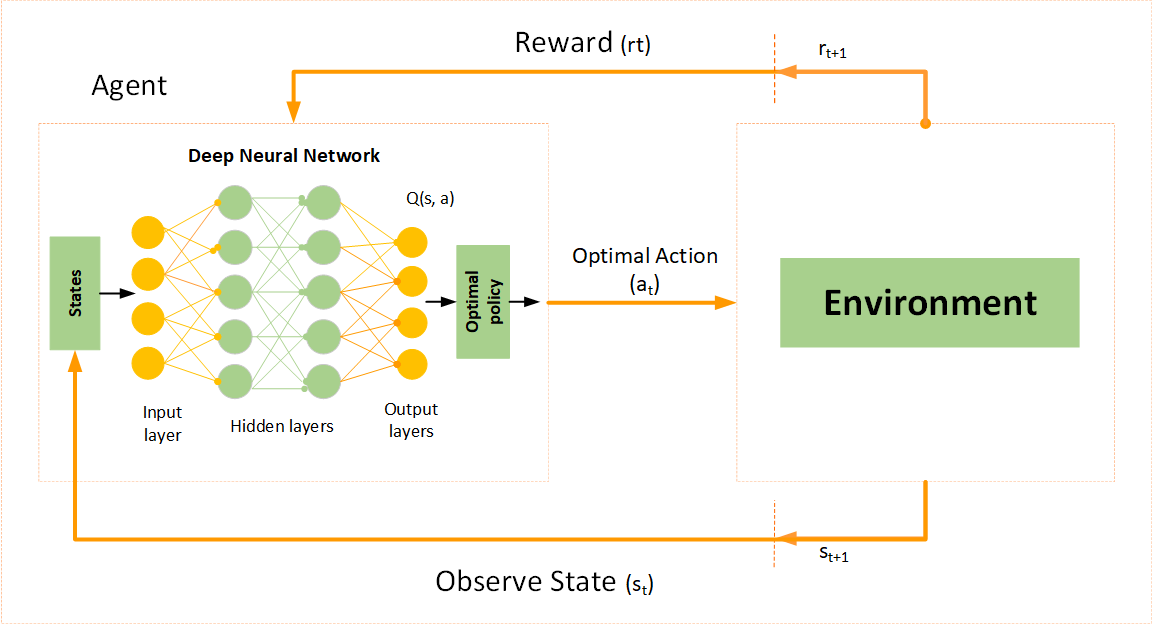
\includegraphics[width=1\textwidth]{img/dqn.png}
    \caption{Illustration of Deep Q-Learning. The Q-network approximates $Q(s, a; \theta)$ using the state as input and outputs a Q-value for each possible action.}
\end{figure}

\subsubsection{Motivation and Overview:}

The goal of DQN is to learn a parameterized Q-function $Q(s, a; \theta)$ that approximates the optimal action-value function $Q^*(s, a)$. This is achieved by minimizing the discrepancy between the current Q-estimate and the target Q-value derived from the Bellman equation.

Unfortunately, Q-learning may suffer from instability and divergence when combined with nonlinear function approximation and bootstrapping. This is particularly problematic when using deep neural networks to approximate the Q-function, due to correlated updates and shifting targets.

\subsubsection{Training Objective and Loss Function:}

At each iteration, the loss function for training the Q-network is defined as:
\[
\mathcal{L}(\theta) = \mathbb{E}_{(s,a,r,s') \sim D} \left[ \left( y^{\text{DQN}} - Q(s, a; \theta) \right)^2 \right]
\]
where the target value $y^{\text{DQN}}$ is:
\[
y^{\text{DQN}} = r + \gamma \max_{a'} Q(s', a'; \theta^-)
\]

Here:
\begin{itemize}
    \item $\theta$ are the parameters of the current Q-network.
    \item $\theta^-$ are the parameters of the \textbf{target network}, a periodically updated copy of the Q-network.
    \item $D$ is the \textbf{replay buffer}, from which mini-batches of experience tuples $(s, a, r, s')$ are sampled.
\end{itemize}

\subsubsection{Key Stabilization Techniques:}

To address the instability issues inherent in combining Q-learning with deep neural networks, DQN incorporates two critical stabilization techniques:

\textbf{Experience Replay:} A buffer that stores past transition tuples $(s, a, r, s')$ \cite{lin1992self}. During training, mini-batches are sampled randomly to break temporal correlations between samples, stabilize updates, and improve data efficiency. Instead of learning directly from consecutive transitions, DQN stores each transition in a replay memory buffer. This approach helps break the correlation between sequential data, improves data efficiency by reusing past experiences, and smooths out the changes in the input distribution.

\textbf{Target Network:} A separate Q-network with parameters $\theta^-$ used to compute the target $y^{\text{DQN}}$ \cite{mnih2015human}. It is updated less frequently (e.g., every $C$ steps), which provides a more stable training signal. By holding the target network fixed for several steps, the moving target problem is mitigated, allowing for more stable Q-value updates.

\textbf{$\varepsilon$-Greedy Exploration:} The agent follows an $\varepsilon$-greedy policy derived from the Q-network. With probability $\varepsilon$, it selects a random action to ensure exploration; otherwise, it chooses the action with the highest estimated Q-value.

\textbf{Gradient Clipping:} In practice, an additional heuristic is applied: the temporal-difference error is often clipped to the range $[-1, 1]$ to prevent exploding gradients. While this clipping breaks smooth optimization and can complicate the theory, it empirically improves convergence and training stability.

\subsubsection{Complete DQN Algorithm:}

\begin{enumerate}
    \item Initialize Q-network with random weights $\theta$.
    \item Initialize target network with weights $\theta^- = \theta$.
    \item Initialize experience replay buffer $D$.
    \item For each episode:
    \begin{itemize}
        \item Initialize starting state $s$.
        \item For each step:
        \begin{enumerate}
            \item Choose action $a$ using $\varepsilon$-greedy policy.
            \item Take action $a$, observe reward $r$ and next state $s'$.
            \item Store transition $(s, a, r, s')$ in $D$.
            \item Sample random mini-batch from $D$.
            \item Compute target Q-value using target network:
            \[
            y_i = r_i + \gamma \max_{a'} Q(s'_i, a'; \theta^-)
            \]
            \item Perform gradient descent step on:
            \[
            \left( y_i - Q(s_i, a_i; \theta) \right)^2
            \]
            \item Every $C$ steps: update target network $\theta^- \leftarrow \theta$
        \end{enumerate}
    \end{itemize}
\end{enumerate}

\subsubsection{Network Architecture:}

The Q-network typically consists of:
\begin{itemize}
    \item An input layer representing the current state $s$ (can be raw pixels or features).
    \item Multiple fully connected or convolutional hidden layers depending on the input modality.
    \item An output layer with $|\mathcal{A}|$ units, each representing the Q-value for an action.
\end{itemize}

\begin{figure}[h]
    \centering
    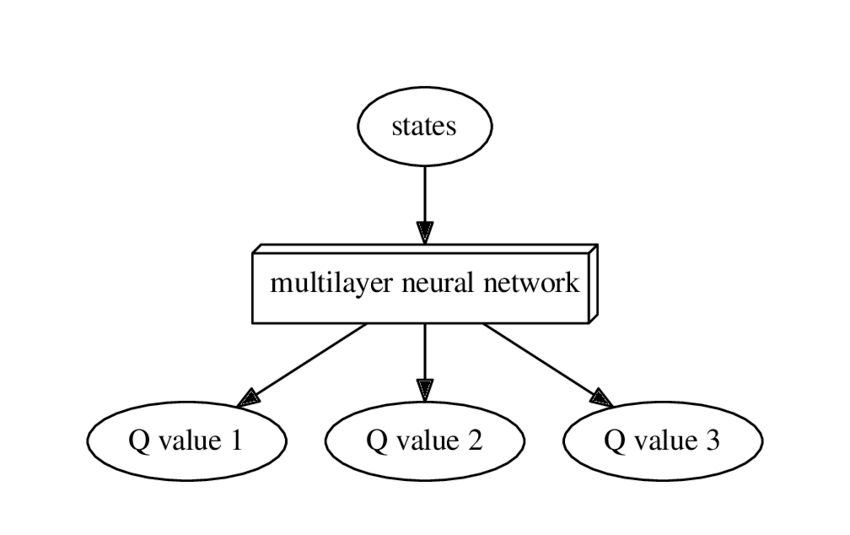
\includegraphics[width=0.7\linewidth]{img/dqn-discrete.png}
    \caption{Q-network architecture for environments with discrete action spaces.}
\end{figure}

\subsubsection{Figure suggestion:} DQN training pipeline showing data flow: environment $\rightarrow$ experience buffer $\rightarrow$ Q-network and target network.

\subsection{Comparative Analysis and Summary}

The table below summarizes the key characteristics of classical RL algorithms:

\begin{table}[h]
\centering
\begin{tabular}{|l|c|c|c|c|}
\hline
\textbf{Method} & \textbf{Model-Free} & \textbf{Bootstrap} & \textbf{Sample Efficiency} & \textbf{Convergence} \\
\hline
Dynamic & No & Yes & High (requires model) & Guaranteed \\
Programming & & & &  \\
\hline
Monte Carlo & Yes & No & Low (needs full& Guaranteed \\
& & &    episodes) & \\
\hline
Temporal Difference & Yes & Yes & Medium & Guaranteed (tabular) \\
\hline
Deep Q-Learning & Yes & Yes & High (with replay) & Not guaranteed \\
\hline
\end{tabular}
\caption{Comparison of classical RL methods}
\end{table}


Each method contributes important ideas and techniques to modern reinforcement learning:

\begin{itemize}
    \item \textbf{Dynamic Programming} provides the theoretical foundation with guaranteed convergence but requires complete environment knowledge.
    \item \textbf{Monte Carlo} methods offer unbiased estimates and can handle non-Markovian environments but suffer from high variance.
    \item \textbf{Temporal Difference} learning combines the best of both worlds with online learning and bootstrapping.
    \item \textbf{Deep Q-Learning} extends these ideas to complex, high-dimensional environments through function approximation.
\end{itemize}

\biblio % Needed for referencing to working when compiling individual subfiles - Do not remove
\end{document}